\documentclass{sigchi}

% Use this command to override the default ACM copyright statement (e.g. for preprints). 
% Consult the conference website for the camera-ready copyright statement.


%% EXAMPLE BEGIN -- HOW TO OVERRIDE THE DEFAULT COPYRIGHT STRIP -- (July 22, 2013 - Paul Baumann)
% \toappear{Permission to make digital or hard copies of all or part of this work for personal or classroom use is 	granted without fee provided that copies are not made or distributed for profit or commercial advantage and that copies bear this notice and the full citation on the first page. Copyrights for components of this work owned by others than ACM must be honored. Abstracting with credit is permitted. To copy otherwise, or republish, to post on servers or to redistribute to lists, requires prior specific permission and/or a fee. Request permissions from permissions@acm.org. \\
% {\emph{CHI'14}}, April 26--May 1, 2014, Toronto, Canada. \\
% Copyright \copyright~2014 ACM ISBN/14/04...\$15.00. \\
% DOI string from ACM form confirmation}
%% EXAMPLE END -- HOW TO OVERRIDE THE DEFAULT COPYRIGHT STRIP -- (July 22, 2013 - Paul Baumann)


% Arabic page numbers for submission. 
% Remove this line to eliminate page numbers for the camera ready copy
\pagenumbering{arabic}


% Load basic packages
\usepackage{balance} % to better equalize the last page
\usepackage{graphics} % for EPS, load graphicx instead
\usepackage{times}  % comment if you want LaTeX's default font
\usepackage{url}   % llt: nicely formatted URLs
\usepackage{listings}
\usepackage{color}
\usepackage[english]{babel}
\usepackage{setspace}

\definecolor{mygreen}{rgb}{0,0.6,0}
\definecolor{mygray}{rgb}{0.5,0.5,0.5}
\definecolor{mymauve}{rgb}{0.58,0,0.82}
\definecolor{black}{rgb}{0,0,0}

\lstset{ %
  backgroundcolor=\color{white},   % choose the background color; you must add \usepackage{color} or \usepackage{xcolor}
  basicstyle=\scriptsize\ttfamily,        % the size of the fonts that are used for the code
  breakatwhitespace=false,         % sets if automatic breaks should only happen at whitespace
  breaklines=true,                 % sets automatic line breaking
  captionpos=b,                    % sets the caption-position to bottom
  commentstyle=\color{mygreen},    % comment style
  deletekeywords={...},            % if you want to delete keywords from the given language
  escapeinside={\%*}{*)},          % if you want to add LaTeX within your code
  extendedchars=true,              % lets you use non-ASCII characters; for 8-bits encodings only, does not work with UTF-8
  frame=single,                    % adds a frame around the code
  keepspaces=true,                 % keeps spaces in text, useful for keeping indentation of code (possibly needs columns=flexible)
  keywordstyle=\color{blue},       % keyword style
  %language=Octave,                 % the language of the code
  morekeywords={*,...},            % if you want to add more keywords to the set
  numbers=left,                    % where to put the line-numbers; possible values are (none, left, right)
  numbersep=5pt,                   % how far the line-numbers are from the code
  numberstyle=\tiny\color{mygray}, % the style that is used for the line-numbers
  rulecolor=\color{black},         % if not set, the frame-color may be changed on line-breaks within not-black text (e.g. comments (green here))
  showspaces=false,                % show spaces everywhere adding particular underscores; it overrides 'showstringspaces'
  showstringspaces=false,          % underline spaces within strings only
  showtabs=false,                  % show tabs within strings adding particular underscores
  stepnumber=2,                    % the step between two line-numbers. If it's 1, each line will be numbered
  stringstyle=\color{black},     % string literal style
  tabsize=2,                       % sets default tabsize to 2 spaces
  title=\lstname                   % show the filename of files included with \lstinputlisting; also try caption instead of title
}

% llt: Define a global style for URLs, rather that the default one
\makeatletter
\def\url@leostyle{%
 \@ifundefined{selectfont}{\def\UrlFont{\sf}}{\def\UrlFont{\small\bf\ttfamily}}}
\makeatother
\urlstyle{leo}


% To make various LaTeX processors do the right thing with page size.
\def\pprw{8.5in}
\def\pprh{11in}
\special{papersize=\pprw,\pprh}
\setlength{\paperwidth}{\pprw}
\setlength{\paperheight}{\pprh}
\setlength{\pdfpagewidth}{\pprw}
\setlength{\pdfpageheight}{\pprh}

% Make sure hyperref comes last of your loaded packages, 
% to give it a fighting chance of not being over-written, 
% since its job is to redefine many LaTeX commands.
\usepackage[pdftex]{hyperref}
\hypersetup{
pdftitle={SIGCHI Conference Proceedings Format},
pdfauthor={LaTeX},
pdfkeywords={SIGCHI, proceedings, archival format},
bookmarksnumbered,
pdfstartview={FitH},
colorlinks,
citecolor=black,
filecolor=black,
linkcolor=black,
urlcolor=black,
breaklinks=true,
}

% create a shortcut to typeset table headings
\newcommand\tabhead[1]{\small\textbf{#1}}


% End of preamble. Here it comes the document.
\begin{document}

\title{DressCode: Tools and Activities to Engage Youth in Algorithmic Craft}

\numberofauthors{3}
\author{
 \alignauthor 1st Author Name\\
  \affaddr{Affiliation}\\
  \affaddr{Address}\\
  \email{e-mail address}\\
  \affaddr{Optional phone number}
 \alignauthor 2nd Author Name\\
  \affaddr{Affiliation}\\
  \affaddr{Address}\\
  \email{e-mail address}\\
  \affaddr{Optional phone number}
}

\maketitle

\begin{abstract}
	Algorithmic craft is the combination of computational design and hand craft for the production of useful, beautiful and personally meaningful physical artifacts. We believe that this combination poses a unique opportunity to engage young people in forms of technological creation in ways that are relevant, pleasurable and intellectually engaging. In this paper we describe our development of DressCode, a software tool that combines programing \emph{and} graphic drawing, enabling the creation of designs that are compatible with handcraft. We evaluated DressCode through a study in which young people created computational designs for screen printing. Our analysis of this study demonstrates useful design principles for combining programing with graphic design and demonstrates the diversity of practices that are possible by engaging people in the creation of objects that are imagined by the mind, designed through computation, and shaped by hand.
\end{abstract}

\keywords{
	Guides; instructions; author's kit; conference publications;
	keywords should be separated by a semi-colon.
}

\category{H.5.m.}{Information Interfaces and Presentation (e.g. HCI)}{Miscellaneous}

\section{Introduction} %clean up to emphasize priorities #1 accessible computational design tools for young people, #2 relevant contexutalization of tools through activity design incorporating craft
There is a growing emphasis on teaching young people skills in technological production to advance our societal technological progress. A common component of these learning initiatives is that they seek to provide students with skills for \textit{future} careers in technology. We believe in the value of working with young people in technological production, but draw upon Dewey's observation that education oriented towards future responsibilities can hinder active participation by students in the present \cite{dewey}. Furthermore, we recoginze that limited participation in STEM fields by women and minorities is partly due to the perception that STEM applications themselves are constrained in cultural and intellectual diversity and breadth \cite{buechley_wild}. To succesfully engage a diverse population of young people in technology-based creation requires two components. First we must develop tools that are accessible and appealing to then.  Second, we must apply these tools to forms of creation that are relevant to their \emph{current} lives and personal interests. Computational design provides an opportune space to achieve these objectives. Prior research has demonstrated that physical craft practices offer a compelling way to engage young people in computation \cite{buechley_comptext},\cite{codeable_objects}. Building off of this work, we explored the application of novice-accessible computational design for craft through the creation of a stand-alone computational design software aimed at young novice programers, and a activity design employing this tool in the production of wearable artifacts.

The process of combining craft and computational design raises several important questions. Foremost, what are important design principles to consider when developing computational design tools for young people? What methods are helpful in ensuring accessibility, creative flexibilty, and support of computational affordances? Furthermore, how can both the software and the activity structure reduce technical and conceptual challenges in translating a computational design into a viable physical artifact? Lastly, what values are reflected in this form of production, what range of young people are engaged by this form of making, and how are the resulting artifacts applicable to their lives?

To explore these questions we have developed our own computational software, DressCode, which features linked editable representations between programing code and graphic drawing and manipulation. In the process of developing DressCode, we prototyped several specific craft activities in sewing, jewelery making and t-shirt design. We used this process as the basis for the development of an activity design which we evaluated in one prelimilary and one long term workshop with highschool students where participants designed and produced jewelery and printed onto clothing. In this paper, we detail the features of the DressCode software, the principles of our computational activity design for young people, and our methodology and results from the workshops. Through analysis of these experiences, we describe design factors that enable young people to computation and making in ways that emphasize pleasure, exploration, intellectual engagement and utility in the service of personal expression. We conclude with a set of recommendations for the development of tools and activities for future forms of engagement in computational design and making.

\section{Creative Opportunities in Computational Design and Craft}
Papert and collaborators recognized early on that computer programing can serve as a way for children to learn powerful ideas about mathematics, geometry and logic \cite{mindstorms}. In computational design, programming provides a powerful way of thinking about design in direct relation to math and logic. Additionally, computational design offers a unique approach to the design process itself. Computational design is best represented as a way of applying procedural thinking to a design task. Designers author rules that define systems capable of producing many outcomes, enabling the production of  multiple design variations that share a set of constraints. Through this systematic abstraction, the following are possible \cite{reas}:
\begin{itemize}
\item \textbf{Precision:} Computation supports high levels of numerical precision.
\vspace{-8pt}
\item \textbf{Visual Complexity:} Computational design allows for rapid creation and transformation of complex patterns and structures, allowing for complex manipulations of numerous design elements.
\vspace{-6pt}
\item \textbf{Generativity:} Designers create algorithms that allow for the computer to autonomously produce unique and unexpected designs.
\vspace{-6pt}
\item \textbf{Parameterization:} Computation allows users to specify a set of degrees of freedom and constraints of a model and then adjust the values of the degrees of freedom while maintaining the constraints.
\vspace{-6pt}
\item \textbf{Remixing:} Computationally generated designs are created by a program which can be modified by other designers. 
\end{itemize}	
%Computational design also contains a number of unique challenges: bring these up in discussion
%\begin{itemize}
%\item \textbf{Formalizing complex problems} As design problems grow in complexity, formalizing the problem in a manner that can be expressed programmatically becomes challenging. 
%\item \textbf{Creating singularities:} A designer will often choose to deviate from a set pattern or structure at specific points in order to create a special emphasis in the area of deviation. Because computational design is governed by a systematized ruleset, the methods of breaking these rules at arbitrary points are often unclear or tedious to implement. 
%\item \textbf{Selecting a final design:} Computational design gives the designer the ability to produce extremely large numbers of solutions to a single design problem. While this is useful in situations where multiple solutions are required, when a single design must be chosen, the process of deciding on a solution is difficult, especially if the decision is based on aesthetic criteria.
%\end{itemize}
\subsection{Challenges in Access and Application}
Although amatuer use of computational design growing, it remains largely inaccessible to individuals who are new to programing. This is in part due to practical and technical barriers. Many of the programming languages used for computational design are difficult for novices to learn and most novice oriented programming environments emphasize producing screen-based work rather than physical objects. Novice-oriented computer-aided-design (CAD) software emphasizes graphic interaction and seldom features computational methods as a key design tool. Significant perceptual barriers also exist. Many people consider programming to be irrelevant to their interests, and are unmotivated to pursue what they perceive to be a highly specialized and difficult undertaking \cite{resnick1}. There also are perceptions of technology in general which may engagement by people who are interested in making. Digital technology is often portrayed as reducing the need or desire for manual human labor, rather than supporting it in creative forms \cite{rosner_craft_vs_design}.

\subsection{Combining Craft and Computational Design}
Despite perceptions of the incompatibility of traditional forms of making and modern technology, craft can be highly compatibile with technologocial production. Craft based approaches offer powerful way to engage young people in computation, and in particular offer the opportunity to reach under-respresented demongraphics like young women. Most frequently, craft has been connected to electronics and physical computing enabling the integration of electronic actuation, sensing and interactivity into craft artifacts \cite{dave}, \cite{kit_of_no_parts}, \cite{jie}, \cite{leah_lilypad}. These combinations have been effective in enaging novice programers and non-traditional user groups. Inspired by this work, we chose to combine craft and computing in a different way, by developing tools to enable the computational design of the visual and physical forms of craft artifacts. We anticipated that this approach would allow for many of the rich properties of craft to be combined with the unique design principles of computational design. The properties of craft we are interested in are as follows:
MAKE THESE SPECIFIC TO HOW THEY EXTEND COMPUTATIONAL DESIGN and factor into our original objectives (relelvancy, accessibility, diversity)
\subsection{Properties of Craft}
\begin{itemize}
\item \textbf{Materiality:} Craft involves working with physical materials by hand. Intuitive decisions are made while physically manipulating the material. 
\vspace{-6pt}
\item \textbf{Pleasure through physical labor:} Fundamental to traditional conceptions of arts and crafts is the idea of pleasure in working with one's hands \cite{abstracting_craft}.
\vspace{-6pt}
\item \textbf{Unification of form and function:} Many forms of craft can applied the creation of objects that merge ornamental and useful qualities.
\vspace{-6pt}
\item \textbf{Craftsmanship:} Traditional notions of craft are closely connected to the idea craftsmanship: the motivation to produce quality work for its own sake \cite{the_craftsman}.
\end{itemize}

\section{DressCode Software Design} %note: describe benefits of learning from multiple reps and add some additional citations.
DressCode is a 2D computational design tool. The primary objectives in DressCode were to reduce the technical challenges of computational design, to support independent and deliberate design decisions through programming. By drawing on the evidence of the benefits of learning environments with multiple representations \cite{ainsworth}, we theorized that providing multiple forms of representation in computational tools would assist novice programers in computational design. DressCode was developed to enable \emph{linked editable representations} of a design in two forms: programmatic and graphic. As users create and manipulate forms graphically, the software generates readable, editable programming statements that correspond to their actions. Users can also generate graphic forms by writing programming statements and manipulate these forms with the graphic editing tools. %DressCode is general purpose, and can be applied to many forms of creation. The software is comprised of a combined integrated development environment (IDE) and a graphic-user-interface (GUI) design tool and a custom programming language and application programming interface (API) (see Figure \ref{fig:auto_generated_code}). Blending the IDE and GUI enabled the development of graphic design tools that work in conjunction with the process of programming. The tools enable graphic drawing and manipulation because the software automatically generates editable code in the IDE that reflects the designer's actions.
\begin{center}
\begin{figure}[h!]
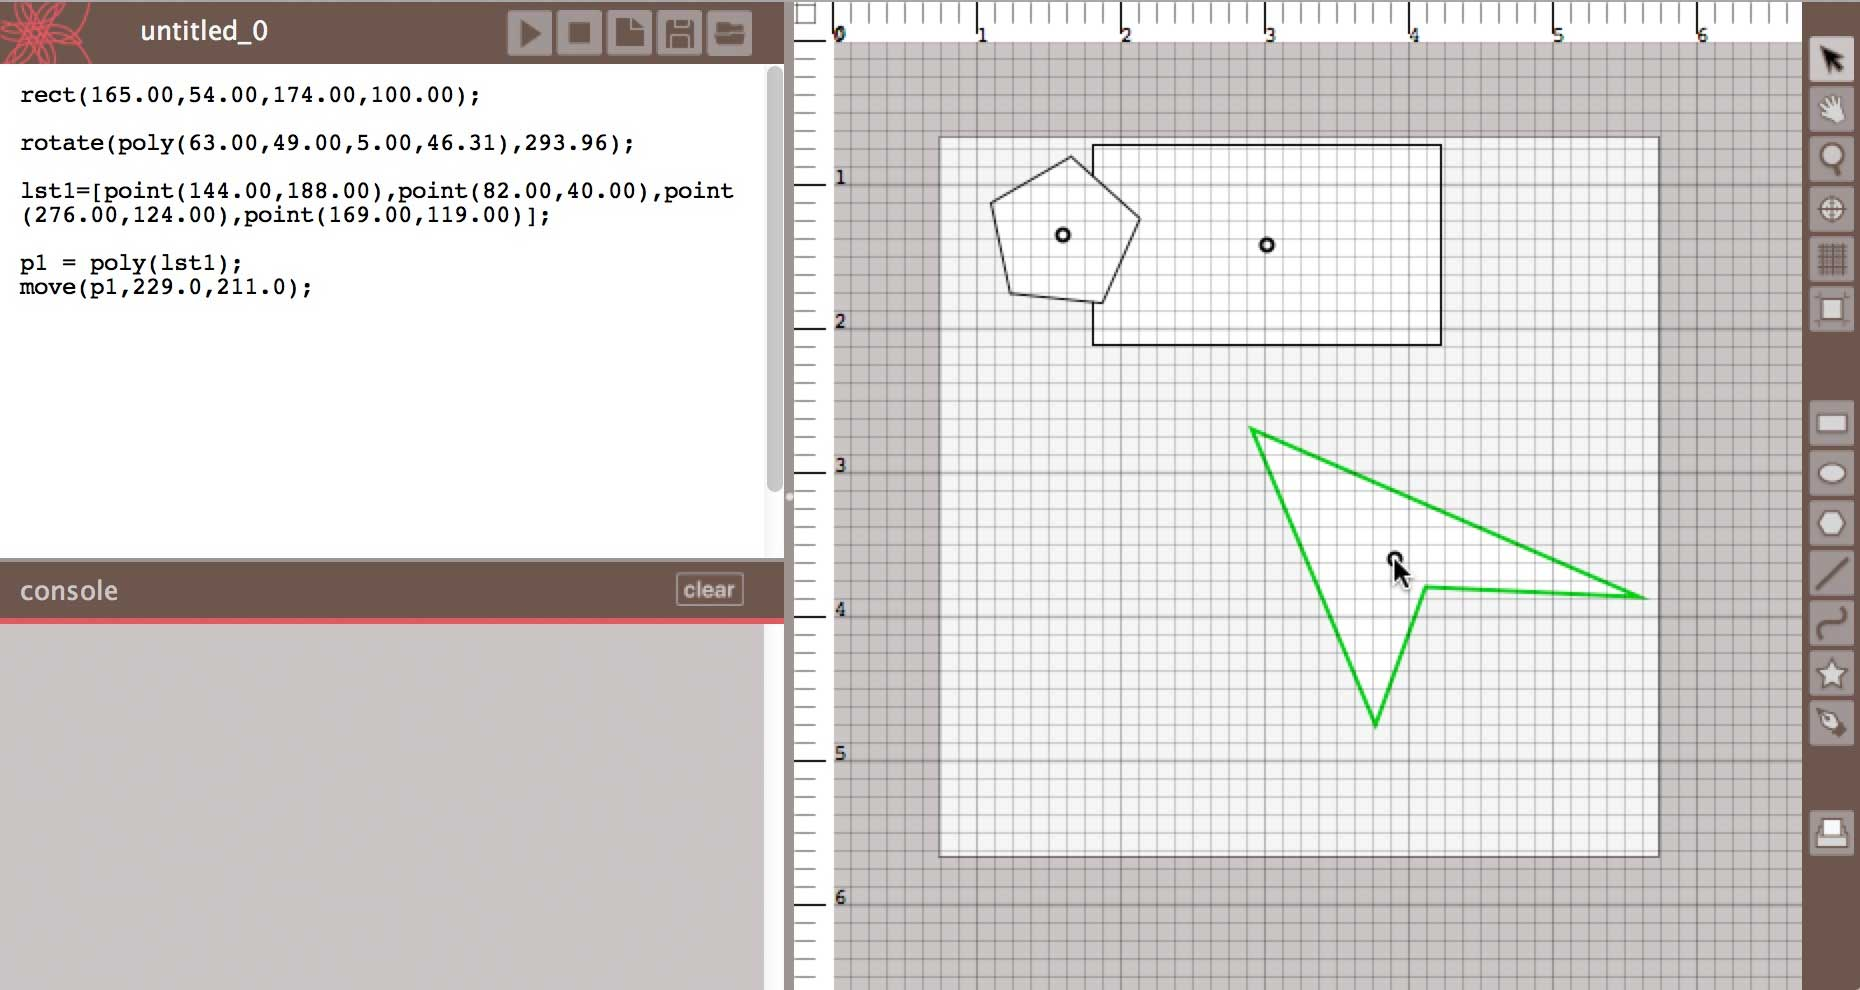
\includegraphics[width=\columnwidth]{images/auto_generated_code.jpg}
\caption{DressCode Software with example of graphically created polygon, rectangle, and irregular polygon, and corresponding automatically-generated code.}
\label{fig:auto_generated_code}
\end{figure}
\end{center}
\vspace{-20pt}
%\begin{center}
%\begin{figure}[h!]
%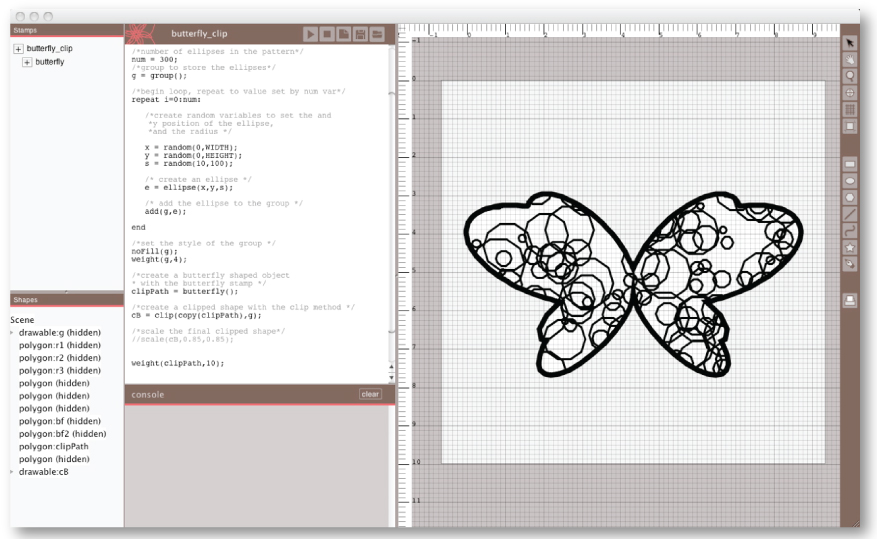
\includegraphics[width=\columnwidth]{images/dresscode_interface.jpg}
%\caption{The DressCode software}
%\label{fig:dresscode_interface}
%\end{figure}
%\end{center}
%\vspace{-20pt}

\subsection{Related Software Tools}
We examined several fields of related software tools in the course of the developing DressCode, including learning-oriented programing environments, accessible CAD tools and prior programing environments with linked graphical editing. Here we discuss notable examples from each category, and describe the disnguising features of DressCode with respect to prior tools.
%Eisenberg and Buechley's research on pervasive fabrication provides a foundation for our objectives in algorithmic craft. Their research encompasses techniques and approaches for incorporating digital fabrication into educational settings, and describes how fabrication enables youth to decorate their environments, allows them to create novel artifacts in the service of personal expression, and stimulates intellectual  \cite{pervasive_fab}. The development of DressCode is closely related to research using the Codeable Objects programming library for youth activities in computation, digital fabrication and fashion design \cite{codeable_objects}. We also examined related software tools: learning oriented programming tools and novel and accessible CAD tools
\subsection{Learning Oriented Programing Environments}
Logo is the seminal novice programming language founded on principles of constructionism and embodiment \cite{papert}. Scratch is one of the most successful modern novice-oriented programming environments, and allows users to create interactive projects by combining command blocks \cite{resnick2}. Processing is a language and development environment for creating complex forms and animations. Described as an entry level programming environment, Processing has also become a successful professional computational design tool\cite{processing}. Processing Logo, Scratch or Processing were explicitly created for compatibility with craft practices, they share features that enable creative programing by novices. To varying degrees, they contain a simplified programming syntax, prioritize visual feedback, and are applicable to a diverse range of projects and interests.

%discuss codeable objects

\subsection{Novel and Accessible CAD tools}
A number of emerging CAD tools blend novel forms of interaction with accessible design mechanisms. Sketch It, Make It is a 2D CAD tool that allows users to constrain their designs through gestures made using a digital drawing tablet \cite{sketchit}. SketchChair enables the design of a chair by sketching with a computer stylus \cite{sketchchair}. FlatCAD connects programming and digital fabrication by allowing users to computationally design construction kits, and fabricate them on a laser cutter\cite{flatcad}. These tools all emphasize various forms of hand engagement in the design process.

In developing DressCode, our goal was to merge the computational functionality of learning-oriented programming environments with the design capabilities of gestural and expressive forms of CAD tools. We did this in a way that allows young people to write code and graphically draw and manipulate forms to produce designs for physical making. 

\subsection{Interface}
The interface of DressCode is divided into a design panel and a coding panel. The design panel contains a resizable drawing board and pan and zoom tools to facilitate navigation. The print tool opens a dialog that allows the user to export their current design in vector format for output through printing, or 2-axis forms of digital fabrication. The coding panel contains a text editor for writing code and an output console for printing output and error reporting. DressCode also contains a declarative listing view, and a stamp menu, discussed in the graphic tools section. When a program is run with the play button, the resulting design is displayed in the design panel.

\subsection{Programming Language and Drawing API}
The DressCode programming language is interpreted with semantic functionality that is simulated through a Java-based library. For most programs, interpretation is instantaneous; however, complex operations require several seconds to be executed. DressCode features a custom textual programming language with native 2D drawing functionality\footnote{A full specification of the DressCode language and API is available at: \url{ommitted for annonymity}}. The language supports conventional programming datatypes as well as drawing primitives in the API. The language is fully featured with support for loops, conditionals and user-defined functions. Variables in DressCode are dynamically typed in order to reduce syntactic challenges for novices. Identifiers can be assigned to datatypes that differ from their original assignment at any point. The language also has built in math and random methods including random noise generation.

The DressCode drawing API is formulated on an Object Oriented Programming paradigm enabling the users to create geometric primitives (points, lines, curves, polygons etc.), and manipulate them as objects. Primitives are initialized by calling the appropriate method and passing it a set of parameters designating the primitive's location and dimensions. There is no ``draw" method for DressCode. All primitives are automatically drawn in the order of their initialization in order to simplify the steps for a design to appear on the screen.
 
Primitives can be modified through two kinds transformation methods, geometric and stylistic. Geometric transformations allow for primitives to be rotated, scaled, moved or combined with other primitives through polygon boolean operations, (union, intersection, either-or and difference), and are performed relative to the origin of the primitive, unless otherwise specified. Stylistic transformations modify the appearance of a primitive (color and stroke weight). Transformations are performed by assigning an identifier to the primitive, and then calling the transformation method with the identifier. By using the transformation methods to manipulate primitives it is possible to generate complex and generative designs from the repetition and structured distribution of simple forms. As a method of organizing sets of primitives, DressCode contains a group datatype, a specialized list for organizing and performing collective transformations on multiple primitives. Groups facilitate more advanced transformations including clipping masks and collective merge operations. 

We created a custom textual programming language for DressCode because we believe textual programming enables transparent representations of computational design algorithms. Because we recognize that textual programming is challenging for novices, we augmented the programming language with visual interaction and feedback in the form of graphic drawing tools.
 
\subsection{Graphic Tools}
\label{subsec:graphic_tools_test}
The graphic tools in DressCode allow users to create and modify elements of their design through graphic selection. The tools maintain a direct symmetry with the DressCode programming language because each tool correspond directly to a method in the drawing API. The use of each tool automatically generates a corresponding textual statement in a user's program. This functionality is designed to encourage natural transitions between graphic drawing and textual programming because it enables elements that are created graphically to be manipulated through textual programming and vice-versa.

\begin{center}
\begin{figure}[h!]

\includegraphics[width=0.75\columnwidth]{images/graphic_tools.jpg}
\caption{The graphic drawing and manipulation tools in DressCode (from left to right: selection and move tool, rectangle tool, ellipse tool, regular polygon tool, line tool, curve tool, SVG import tool, pen tool)}
\label{fig:graphic_tools}
\end{figure}
\end{center}
\vspace{-20pt}

The toolset includes regular primitive creation tools and a pen tool for the creation of irregular forms (see Figure \ref{fig:graphic_tools}).  In addition to the drawing tools, the selection tool allows for individual primitives and groups to be manually selected and moved. When a primitive is moved for the first time, a textual move statement is inserted into the user's program. For all subsequent moves of that primitive with the move tool, the inserted move statement is updated to reflect the new coordinates of the primitive (see Figure \ref{fig:auto_generated_code}).

%\begin{center}
%\begin{figure}[h!]
%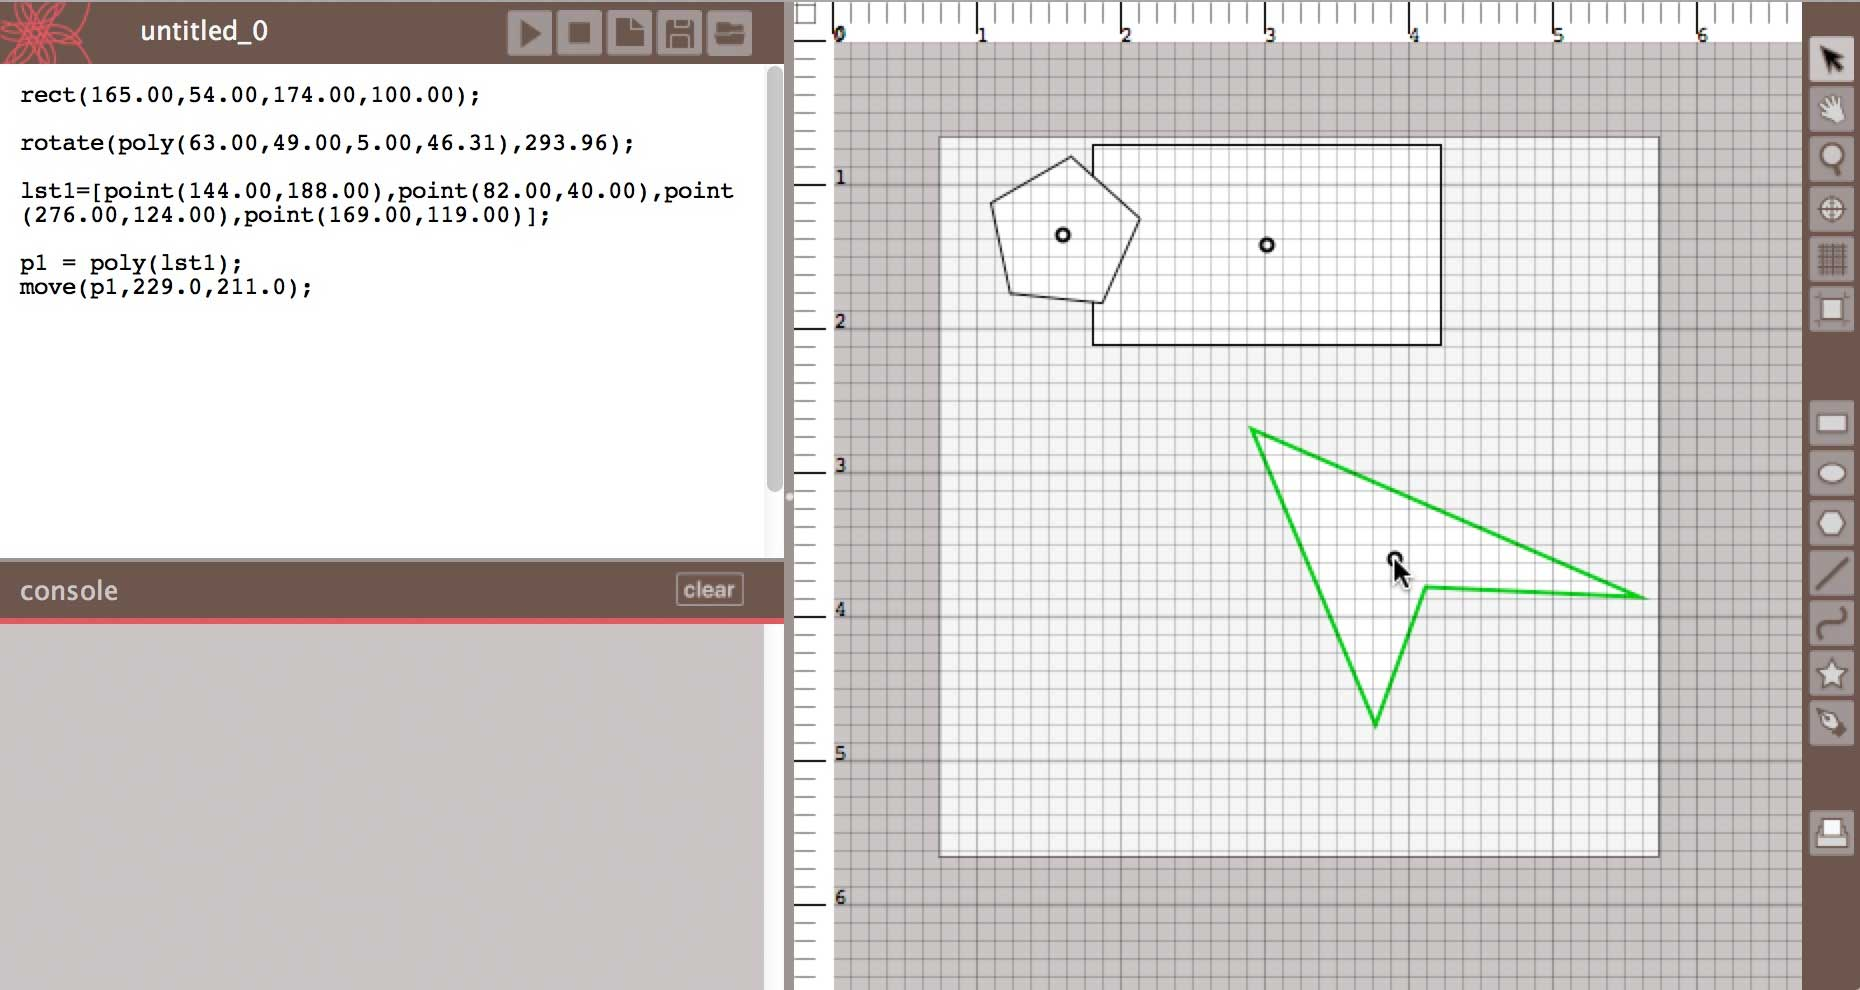
\includegraphics[width=\columnwidth]{images/auto_generated_code.jpg}
%\caption{Graphically created polygon, rectangle, and irregular polygon, and corresponding automatically-generated code. (The irregular polygon has just been moved with the selection tool.)}
%\label{fig:auto_generated_code}
%\end{figure}
%\end{center}
%\vspace{-20pt}

The declarative view contains a listing of all primitives in the current design. Child primitives are nested within their parent groups. When selected in the declarative view, the primitive is selected and highlighted in the design view, and the line where the primitive was last modified in the text-editor is highlighted (see Figure \ref{fig:declarative_view}). The declarative view is designed to provide visual feedback on how elements of a design connect to the user's program, and provide a practical selection technique for complex designs.

\begin{center}
\begin{figure}[h!]
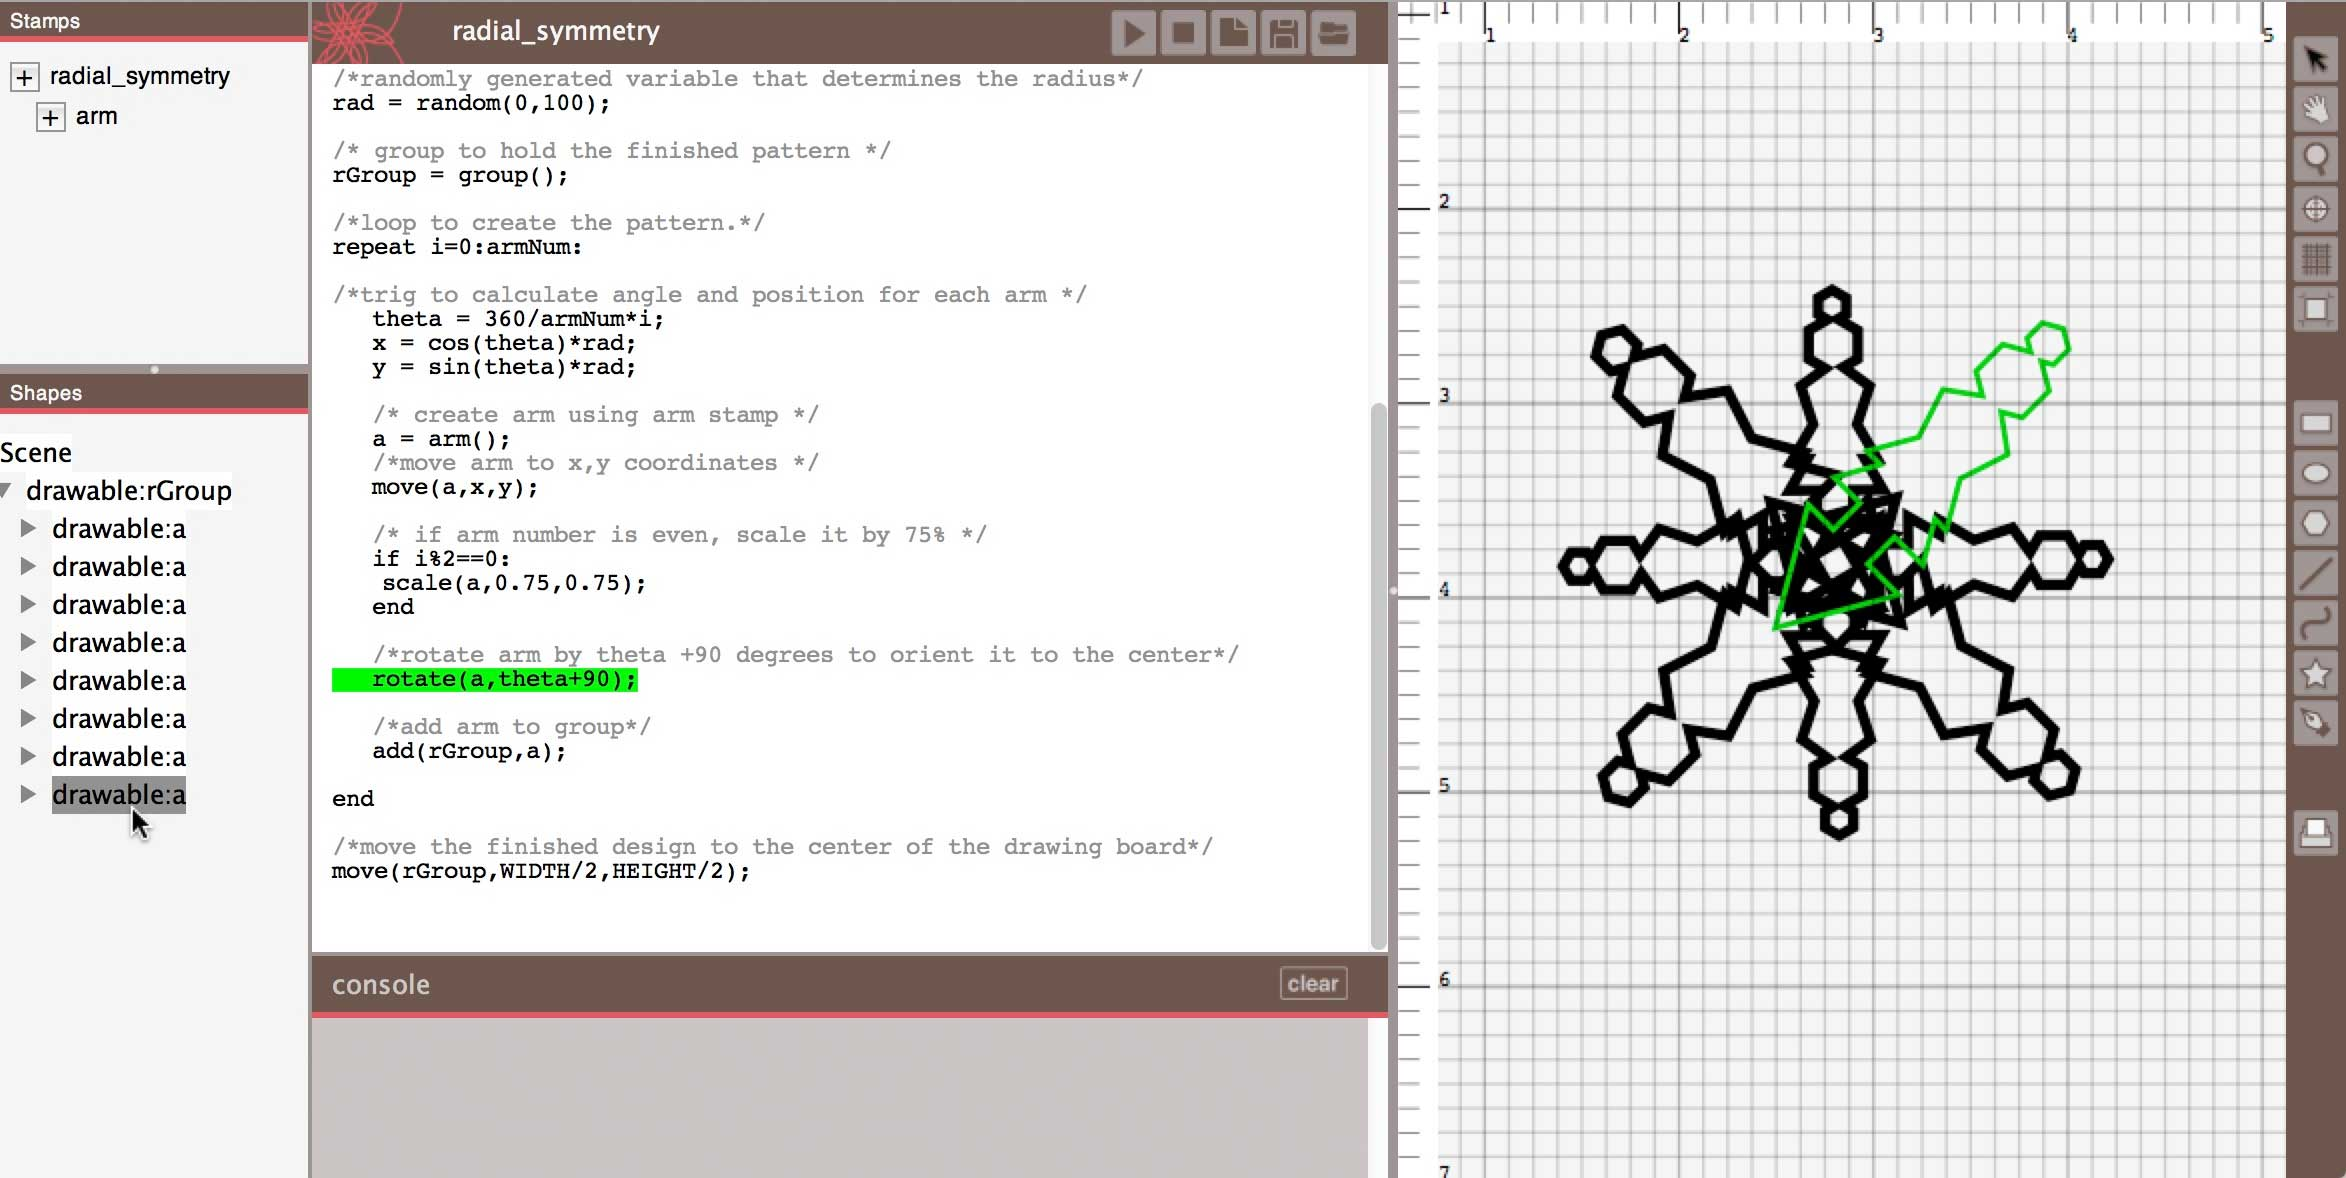
\includegraphics[width=\columnwidth]{images/selection_mechanism.jpg}
\caption{Declarative view with selected primitive}
\label{fig:declarative_view}
\end{figure}
\end{center}
\vspace{-20pt}

DressCode contains functionality to help people organize their code in the form of static and dynamic \textit{stamps}: graphically created functions that return shape primitives. Dynamic stamps are created by selecting a portion of code in a user's program and then selecting the dynamic stamp option from the menu. A dynamic stamp will package the selected code in a function with a name specified by the user. Static stamps are created by graphically selecting a single primitive or group with either the selection tool or the declarative view, and selecting the static stamp option. Static stamps translate shapes generated in random positions to explicit primitives, allowing users to save a specific instances of a generative design (see Figure \ref{fig:stamps}).
Stamps are listed in the stamp menu and can be added to a user's primary program by selecting the \textit{+} icon next to each stamp. The code of both static and dynamic stamps can be modified by the user as the code generated is human readable.

\begin{center}
\begin{figure}[h!]
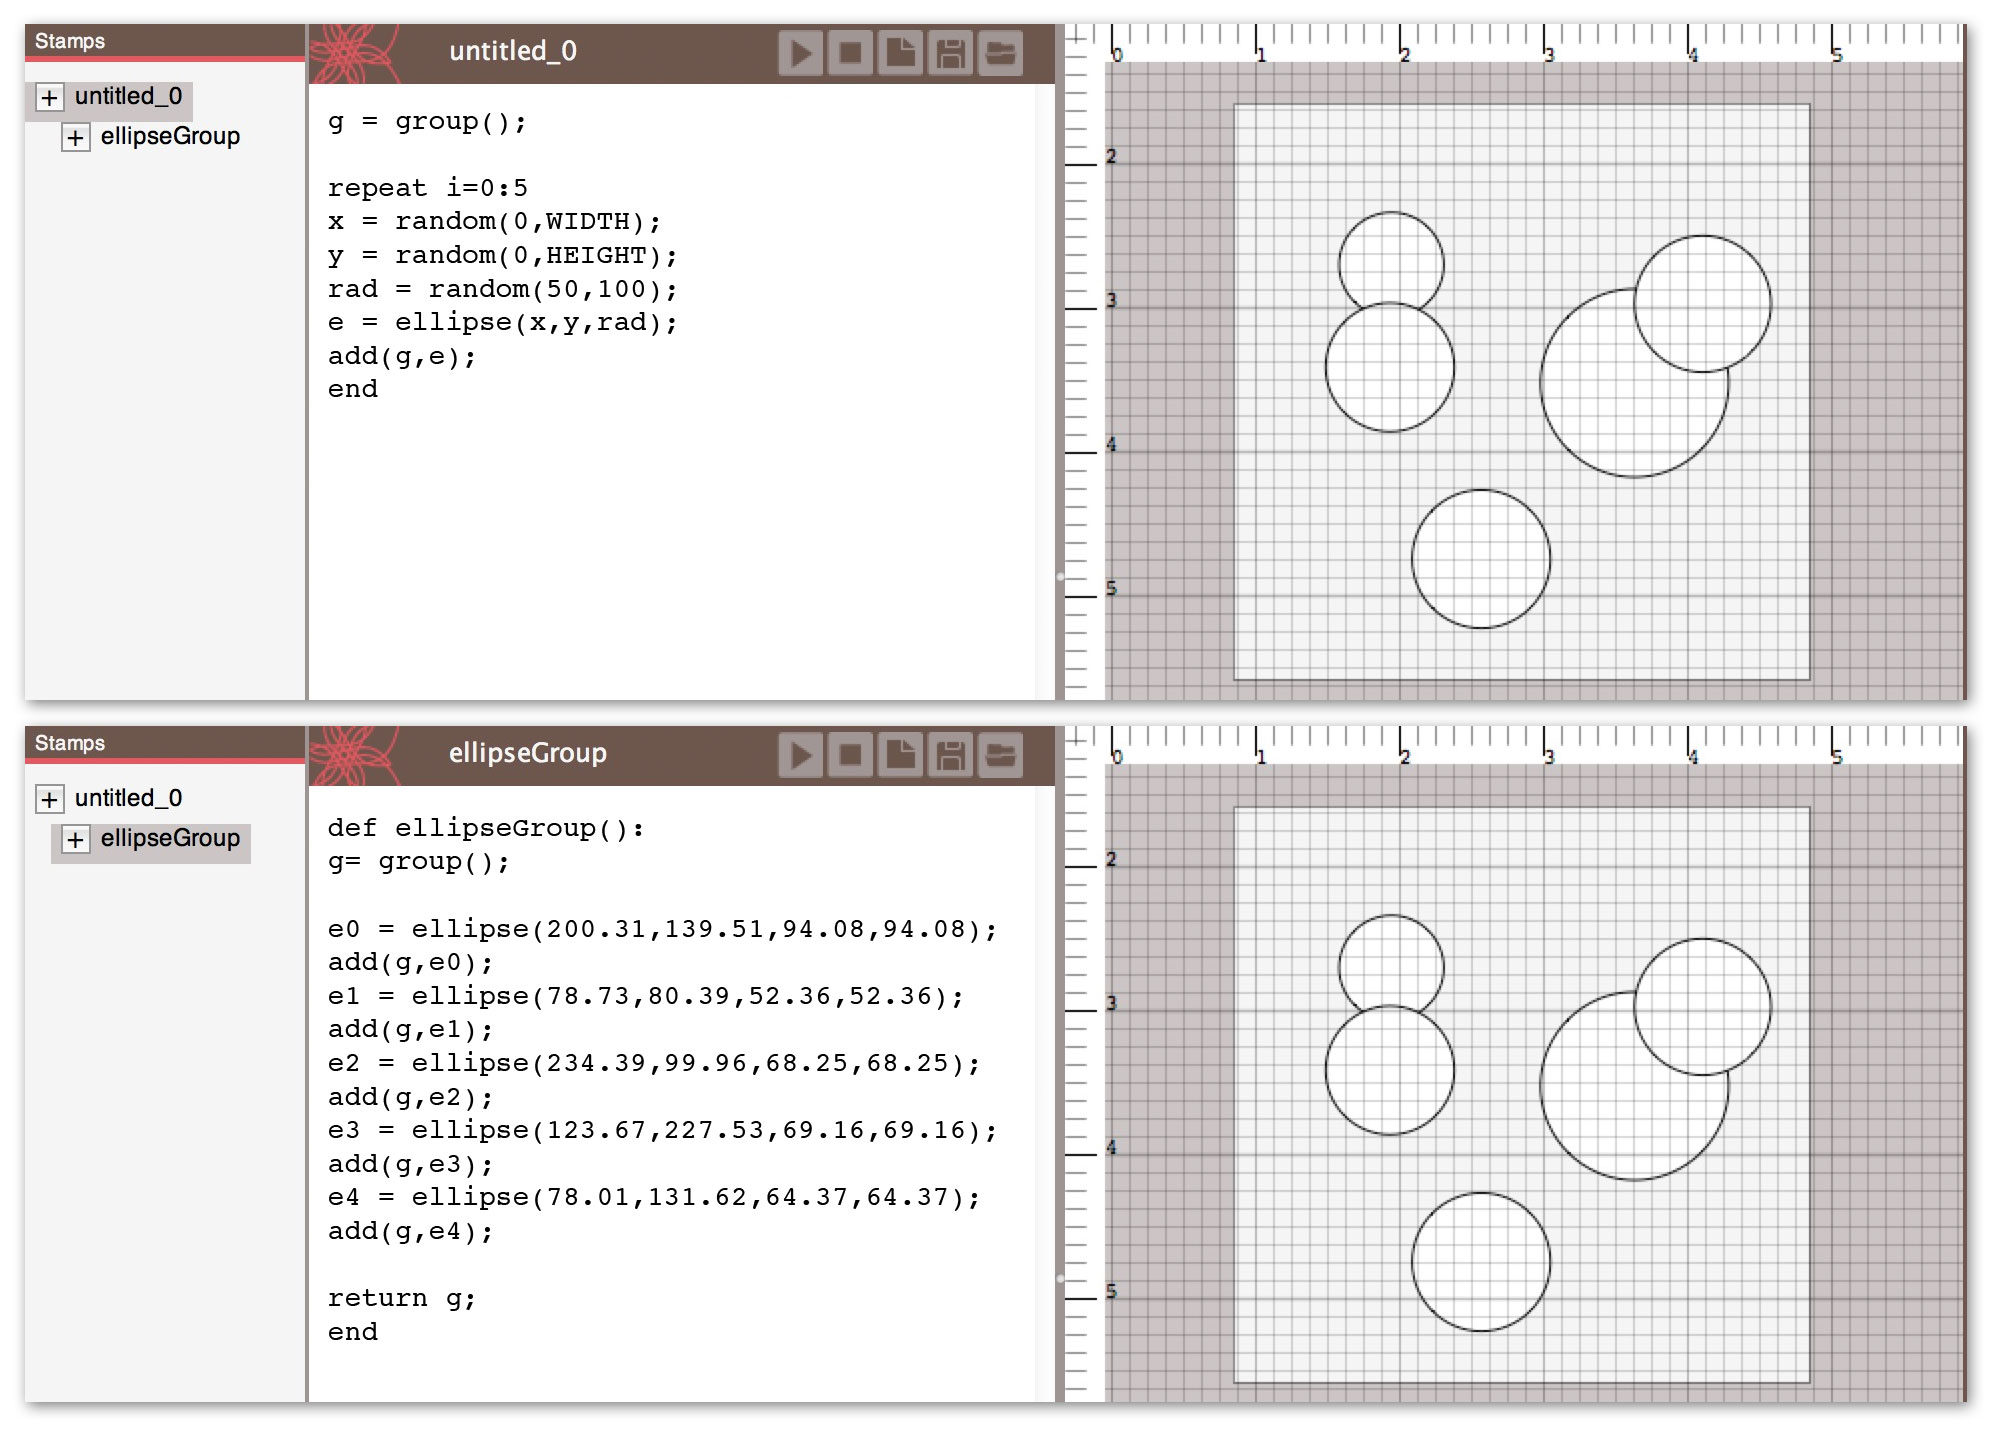
\includegraphics[width=\columnwidth]{images/stamps.jpg}
\caption{Static stamp functionality. (Top: User defined code which generates five random ellipses. The ellipses' positioning and size will change each time the program is run. Bottom: static stamp created from ellipses which will always return the same design.)}
\label{fig:stamps}
\end{figure}
\end{center}
\vspace{-20pt}

\section{Activity Design}
Domain-specific software is an important component of engaging youth in algorithmic craft; however it is equally important to appropriately design the context in which the software is applied. In this section, we discuss the primary components of our activity design using DressCode: \emph{learning, creation and reflection}. These components are directly influenced by the Brennan and Resnick's dimensions of computational thinking\cite{computational_thinking}, but are specific to algorithmic craft.

\subsection{Learning}
Learning components of activities relate to participants' understanding of the core affordances of computational design and the values of craft. Computational learning in algorithmic craft entails learning programming concepts and understanding how they relate to design objectives. Craft learning involves learning technical craft practices and evaluating designs in respect to these practices.

\subsection{Creation}
Creation in algorithmic craft is comprised of \emph{iteration and repetition}, \emph{remixing}, and \emph{critique}. In computational design, iteration occurs as designs evolve through incremental steps. Craft involves repetition, where successful execution requires practice of manual skills. Remixing plays a key roles both in computational design and craft. In computational design example programs serve as starting points for novices and existing designs are merged to produce something new. In craft people share parts and techniques and produce multiple variations of a design.

\subsection{Extension}
Algorithimic craft emphasizes extension through \emph{reflection, sharing and connection}. Reflection occurs as practitioners examine and evaluate their creations. Sharing extends reflection as practitioners share the process behind their artifacts with friends and family. Connection occurs when the experience of one project generates ideas for future pursuits.

\section{User Study}
To better understand young people's practices in algorithmic craft, and evaluate the effectiveness of DressCode, we conducted an algorithmic craft activity using DressCode as the primary tool. The activity consisted of a four-day workshop, divided between two consecutive weekends, in which participants created computational designs in DressCode and screen-printed them onto t-shirts.

\subsection{Evaluation Methods}
The participants' experiences were evaluated through written surveys and group discussions. Pre-workshop surveys focused on participants' previous experience and attitudes towards programming, craft and design. Post-workshop surveys contained attitudinal questions that were matched to the pre-surveys, as well as a range of written questions asking the participants to describe their process and project. Interim surveys were also administered following the first two days, and asked participants about their experiences using the DressCode software. We held three group discussions with the participants which were recorded and transcribed. The discussions examined participants' design process, experience using DressCode in combination with craft practices, and ideas they had for modifying or augmenting future activities and software tools. Survey results, verbal discussion responses and project outcomes were analyzed to identify repeated and notable elements of participants experiences, and how they connected to our original research objective of helping people connect to computation in ways that are relevant, personally meaningful and intellectually engaging.

\subsection{Demographics of Participants}
The screen printing workshop was conducted among 7 young adults, aged 13-17, and one older participant, aged 21. Three participants were male, and five were female. Participants were selected to represent a range of programming, craft and design experience (table \ref{table:experience}).
\begin{table}
  \centering
  \begin{tabular}{|c|c|c|c|c|c|}
    \hline
    \multicolumn{1}{|p{0.75cm}|}{\centering\tabhead{}} &
    \multicolumn{1}{|p{1.3cm}|}{\centering\small{no experience (1)}} &
    \multicolumn{1}{|p{0.75cm}|}{\centering\small{2}}&
    \multicolumn{1}{|p{0.75cm}|}{\centering\small{3}}&
    \multicolumn{1}{|p{0.75cm}|}{\centering\small{4}}&
    \multicolumn{1}{|p{0.75cm}|}{\centering\small{expert (5)}}\\
    \hline
    \small{art} & 0 & 0 & 4 & 4 & 0\\
    \hline
    \small{craft} & 1 & 0 & 3 & 4& 0  \\
    \hline
	\small{programming} & 1 & 1 & 4 & 1& 1  \\
    \hline
	\small{design} & 0 & 2 & 3 & 3& 0  \\
    \hline
  \end{tabular}
  \caption{Prior participant experience. (Numerical values in the columns correspond to the number of participants with that response.)}
\label{table:experience}
\end{table}
\subsection{Workshop Progression}
Prior to the workshop, we had participants select t-shirts in a size and color of their preference. In the first session of the workshop, we introduced participants to generative design and programming in DressCode by guiding them through writing their own random walk algorithms that produced patterns composed of lines. We followed by explaining the graphic drawing tools, and had participants modify their random walk patterns by incorporating shapes they created graphically. The following session began with an overview of photo emulsion screen printing and transitioned to computational design activities. We demonstrated several other forms of generative design by providing participants with images of sample designs and having them work in groups to write a set of instructions to re-produce the design. As a group we discussed their results, and looked at code examples in DressCode that would produce results similar to the samples.  %(figure:\ref{fig:example_designs}). 
%\begin{center}
%\begin{figure}[h!]
%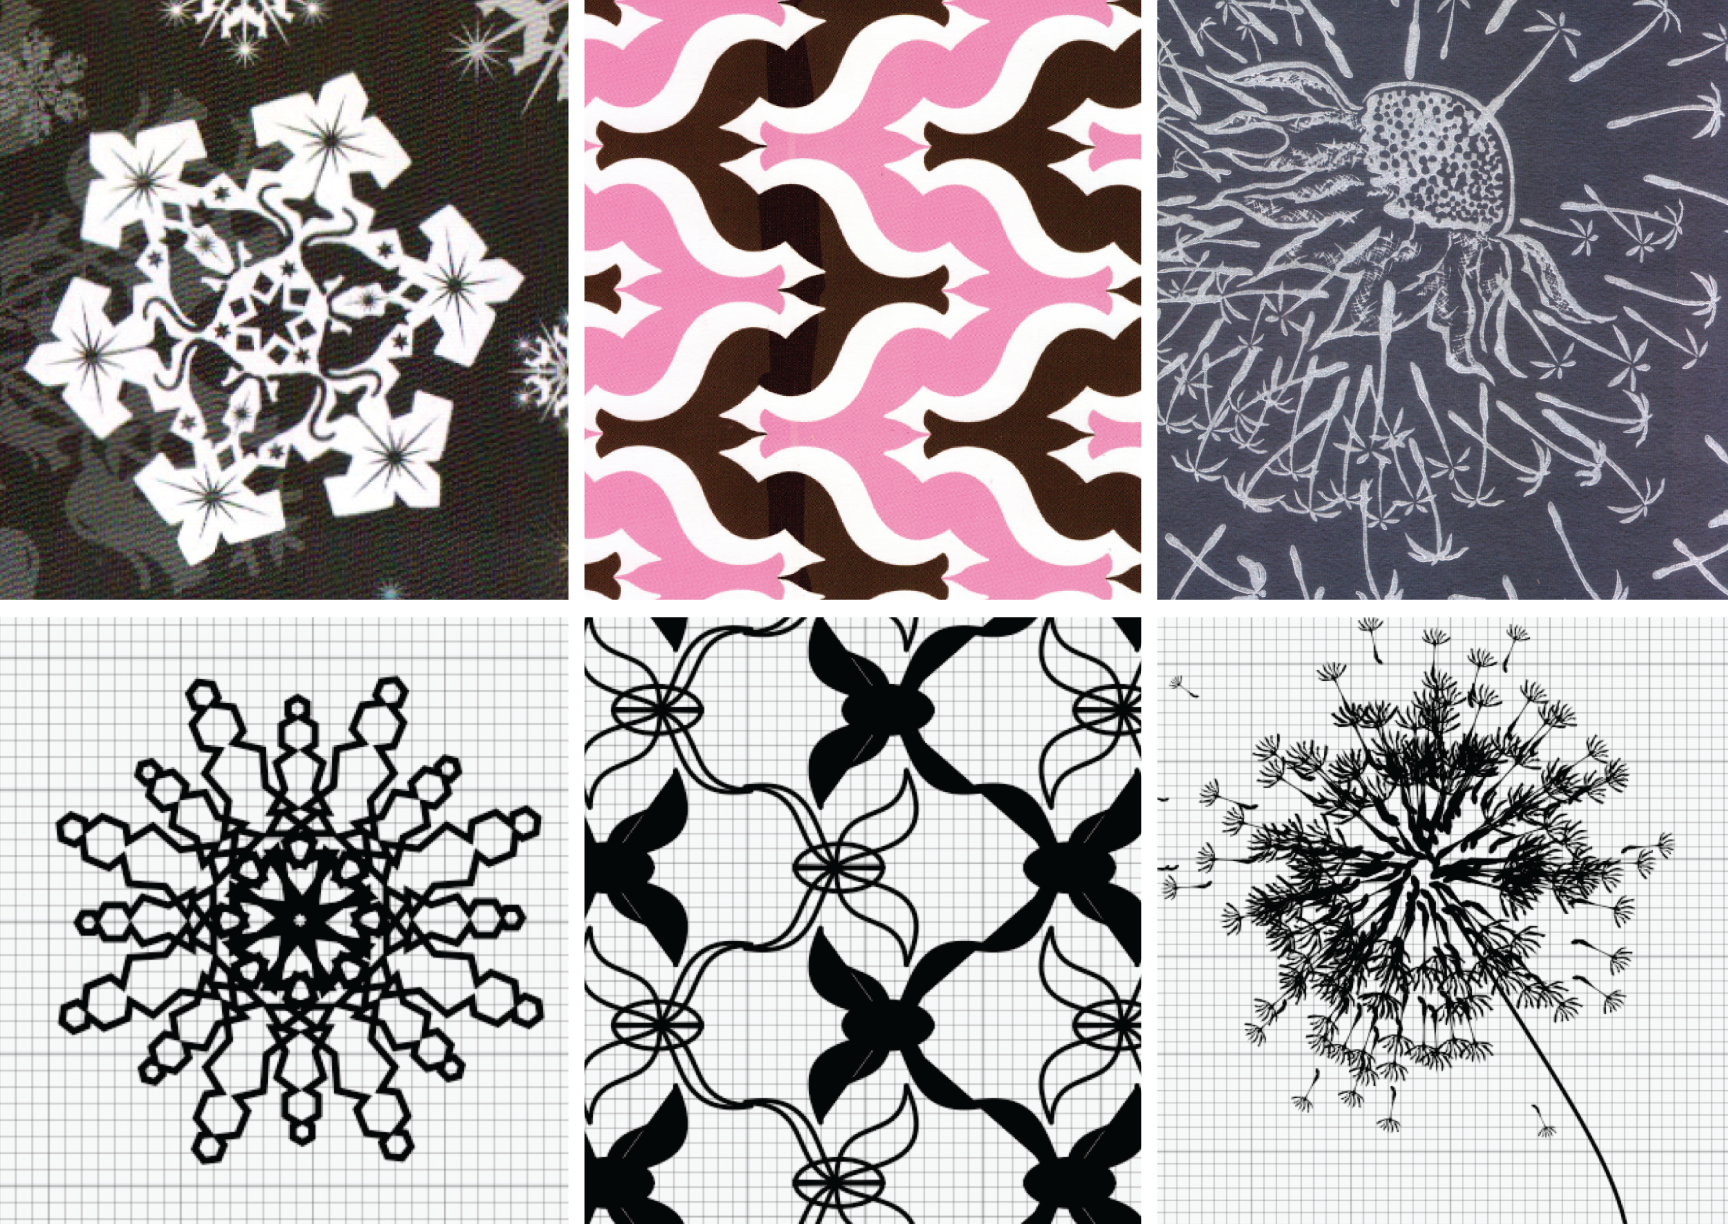
\includegraphics[width=\columnwidth]{images/pattern_examples.png}
%\caption{Sample designs and corresponding examples in DressCode}
%\label{fig:example_designs}
%\end{figure}
%\end{center}
%\vspace{-20pt}
Participants were given the task of creating a computational design to screen print onto a t-shirt they would want to wear, and given 4-5 hours open design time divided between two days. Other portions of the workshop were spent preparing screens for screen printing. Participants laser-printed their finished designs on transparencies, which the instructors exposed on the screens overnight (see Figure \ref{fig:screen_printing_process}). On the last day, participants practiced screen printing and printed their final designs onto their shirts.
\begin{center}
\begin{figure}[h!]
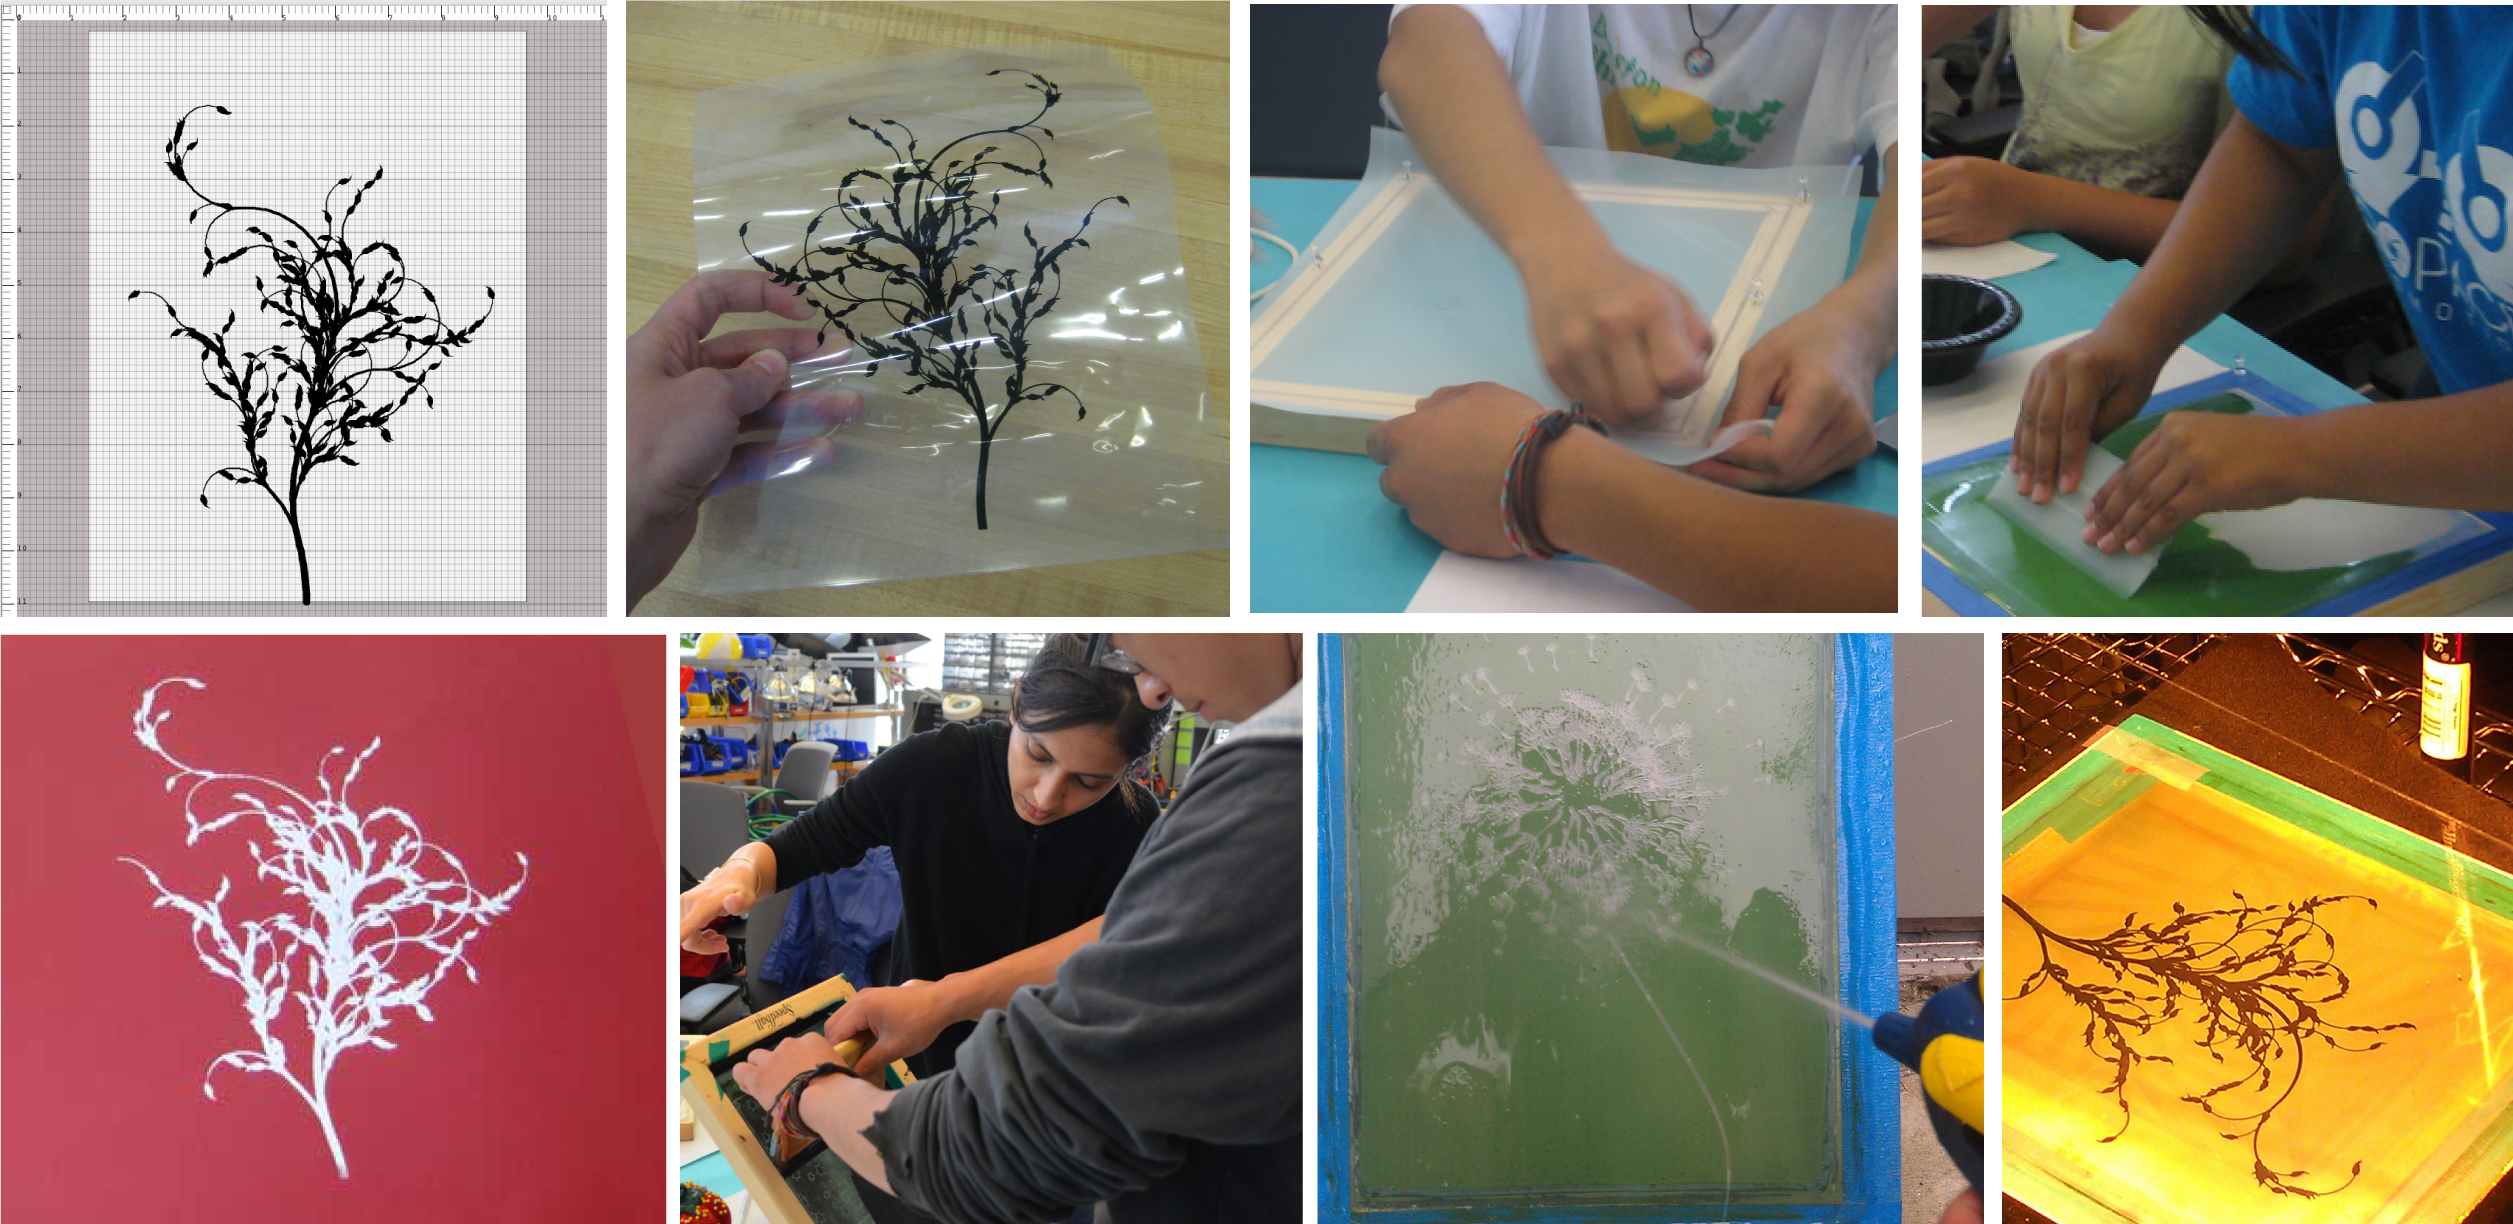
\includegraphics[width=\columnwidth]{images/screen_printing_process.png}
\caption{Screen printing process. (Clockwise from upper-left: Digital design, printed transparency of design, stretching the screen, applying photo emulsion, exposing the screen with the transparency, washing out the screen to reveal the design, printing with the finished screen, a completed print.) }
\label{fig:screen_printing_process}
\end{figure}
\end{center}
\vspace{-20pt}

\subsection{Screen Printing Results}
Each participant in the workshop was successfully able to use DressCode to produce a design for their t-shirt (see Figure \ref{fig:screen_results}). The design approaches among the participants varied. Two participants created designs that were derived from their random walk algorithms, one participant created a pattern by combining two of the example patterns and making adjustments, and one participant worked solely by modifying an example. Other participants designed patterns independent of the examples, including a generative landscape, a geometric spiraling pattern and a complex radial pattern comprised of overlapping lines. The screen printing process was extremely popular among the participants. Each person successfully created their own screen through photo-emulsion transfer, and mastered the basics of printing. Several participants not only printed to the provided shirts, but also brought in additional garments to print on for friends and family. The participants requested to keep their screens following the workshop, and stated on the survey that they planned to continue making prints for themselves and others. All participants indicated that they planned to wear their shirts, and two participants contacted us via email following the workshop thanking us for the experience, and requesting tips on how to properly care for their garments. 

\begin{center}
\begin{figure}[h!]
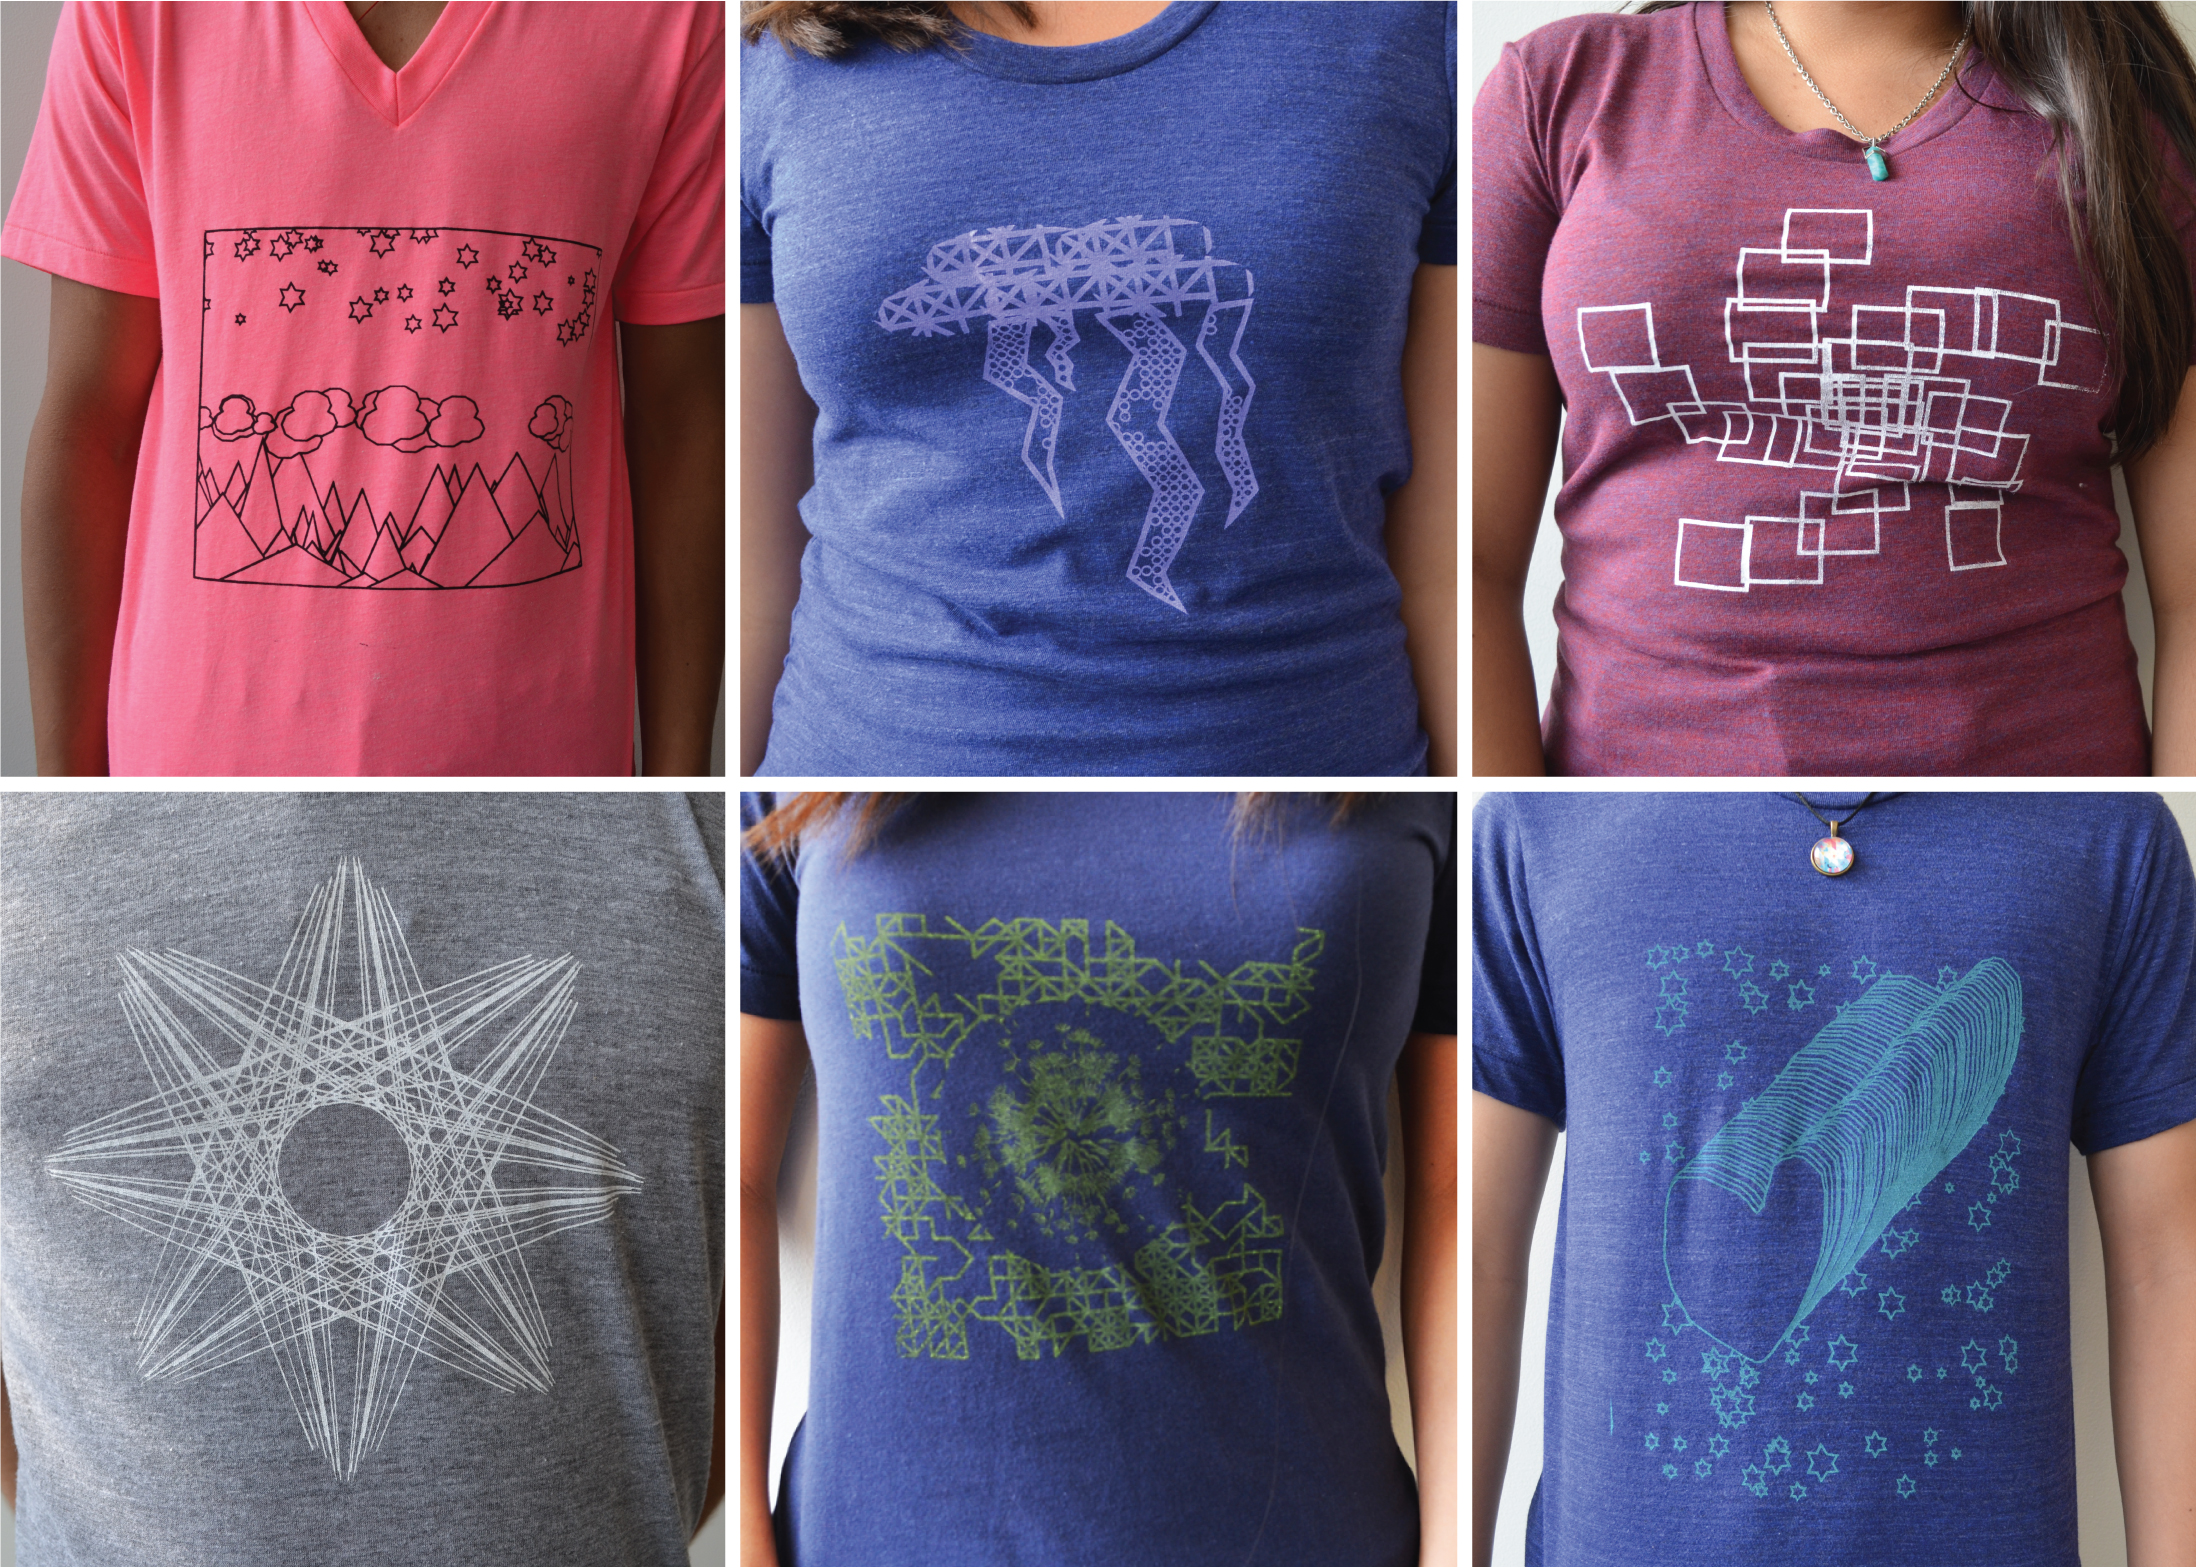
\includegraphics[width=\columnwidth]{images/shirt_results.jpg}
\caption{Some of the completed shirts. (Clockwise from upper-left: generative landscape, clipping mask cloud pattern, geometric spiral, random walk of hand-drawn hearts, dandelion-random walk mashup, generative linear-radial pattern.) }
\label{fig:screen_results}
\end{figure}
\end{center}
\vspace{-20pt}

An evaluation of the pre, mid and post-workshop surveys demonstrated that following the screen printing, participants attitudes towards programming, design and craft, changed from what they were after the computational design sessions. In the majority of cases, this change was positive; participants indicated greater interest in learning programming in the future, a stronger belief that programming was a tool that they could create things they would use in their daily life, and greater comfort in programming on their own following the craft activity. Participants were positive about the graphic tools, although they requested that their functionality be extended to incorporate a greater range of transformation methods. All participants said they would be interested in using DressCode for another activity, and all but one indicated they would like to continue using the programming language in particular.

\section{Discussion}
In our discussion of the workshops we focus on three primary elements. We evaluate the successes and limits of the DressCode software, with an emphasis on how people used the graphic drawing and manipulation functionality. Second, we examine participant's design practices and discuss how they connect to the affordances of algorithmic craft. Third, we consider what participants accomplished in the workshop by evaluating how the completed artifacts resonated with the participants' personal values and lives.

\subsection{Combining Graphic Manipulation and Textual Programing}
	One of our primary research objectives was to develop techniques that were accessible while also supporting personal aesthetics and styles through computational design. Analysis of participants' use of DressCode indicates that for many people, the graphic tools were helpful in this regard (table \ref{table:graphic_tools}). 

\begin{table}
  \centering
  \begin{tabular}{|c|c|c|c|c|c|}
    \hline
    \multicolumn{1}{|p{0.75cm}|}{\centering\tabhead{}} &
    \multicolumn{1}{|p{1cm}|}{\centering\small{str. disagree}} &
    \multicolumn{1}{|p{0.8cm}|}{\centering\small{disagree}}&
    \multicolumn{1}{|p{0.8cm}|}{\centering\small{neutral}}&
    \multicolumn{1}{|p{0.8cm}|}{\centering\small{agree}}&
    \multicolumn{1}{|p{0.8cm}|}{\centering\small{str. agree}}\\
    \hline
    \small{helped create design} & 0 & 1 & 1 & 3 & 2 \\
    \hline
    \small{helped understand program} & 0 & 0 & 5 & 3& 0  \\
    \hline
  \end{tabular}
  \caption{Participant survey responses on the role of graphic tools. Numerical values in the columns correspond to the number of participants with that response.}
\label{table:graphic_tools}
\end{table}

Before the graphic tools were formally introduced, several participants independently started experimenting with them on their own. Several people also indicated that the graphic drawing tools also helped them to better understand the process of writing their program. Participants expanded on this idea during the discussion:
\begin{quotation}
\textit{You find a tool, you draw on the canvas and it shows you the code, that's basically it.}
\\Participant Z
\end{quotation}

\begin{quotation}
\textit{I think that having the drawing tools and having it also show the code there makes it so that you can see as you're doing it. [By] having a graphical side and having it auto update the code, it can show you that you want to work with the code you're learning as you're using the GUI. So that people could try and say ok, if I can't do something with the graphical tools, let me try and manipulate the code. And then you already have some understanding because you've been using the graphical tools and it's been appearing over there the entire time.}
\\Participant B
\end{quotation}

A visual examination of many of the finished products in the workshop demonstrates the impact the graphic drawing tools on the aesthetics of the designs (see the heart and cloud designs in Figure \ref{fig:screen_results}). The pen, and shape generation tools allowed participants to blend their personal drawing styles with computational elements, resulting in computational forms that reflected the drawing techniques of the creator. 

The introduction of the graphic tools also resulted in a discussion among participants about future paradigms for graphic design and programming. Participants unanimously agreed on the utility of the drawing tools, but requested that they be developed further to provide more sophisticated forms of drawing, control, and visual feedback. In contrast to the popularity of the drawing tools, several participants had difficulty with the move tool. From a development perspective, the move tool was challenging to implement because there were numerous ways it could be represented in code. We implemented what we felt to be the simplest option (inserting a move statement for primitives with identifiers, or wrapping the declaration statement of un-identified primitives), but doing so required us to speculate about what would be most useful and intuitive for novice programmers. In practice, participants who had large numbers of primitives in their programs without identifiers found the move behavior confusing because it modified an existing statement in their program, rather than generating a new line of code. This confusion makes it clear that we should re-consider the functionality of the tool, however it also points to a design principle for future tools. The fewer assumptions a tool has to make about the intentions of the user, the less likely it is that it will conflict with the user's coding and design process. We feel the creation of more sophisticated primitive generation tools is a form of low hanging fruit that will provide immediate benefits to the user's design process, whereas transformation tools require greater analysis on how to be implemented effectively. 

Participants responses in the discussion also demonstrated ways in which the tools had expanded their comprehension of the computational design process. One participant suggested adding an graphic erasing tool, which resulted in a conversation on how such a tool could be implemented:

\begin{quotation}
Participant Z: \textit{So if you erase one line, it becomes two lines...so it's going to generate the code for two lines?}
Participant M: \textit{No like if you drew a line with the sidebar, and then you decided you didn't like, you don't have to go to the code, erase it and press play, you could just take the erase tool, click on it and then it goes away.}
Participant Z:  \textit{No, what I mean is like if you just wanted to erase half?}
\end{quotation}

This conversation reinforces issues when making assumptions about individuals' design processes in the implementation of graphic tools. Moreover, this discussion shows the participants actively considering how new graphic tools could correspond to writing code. Conversations of this nature demonstrate how graphic tools can stimulate thinking about computational processes for young programmers, rather than making them opaque. During the workshop, a similar discussion occurred around the topic of preserving generative forms. Participants had different ideas for preseving static instances of randomly generated designs. Several participants used the static stamp tool for this purpose, but others requested different forms of control over the randomly generated values. One participant wondered if he could have the software store the randomly created values for a specific program, and allow the user to specify the point at which new values would be generated. Building on this idea, we asked participants if they would have preferred to specify random noise generation through a form of graphic input similar to the graphic dialog tools, or if they felt creating random methods in the programming environment was useful. Two participants said they would prefer that as an option, however others disagreed, stating that they felt you would lose some of the functionality of the program in the process.
\begin{quotation} 
\textit{Well that would kind of take away from the programming part of it, because you'd be trying to turn everything into a UI.
The important thing I really feel about DressCode is you can make things random, these are drawn (indicating a hand drawn graphic) and these are from the programming part (indicating the random repetition of the graphic).}
\\Participant Z
\end{quotation}

Understanding the creative potential of one's tools is essential for effective design. It is encouraging therefore, that many participants not only saw the value of the graphic tools, but also understood and embraced the applications of textual programming in combination with these tools.  

The introduction of graphic manipulation tools in conjunction with textual programming demonstrated several conclusions. Drawing tools proved to be largely intuitive and easy to use and they allowed participants to blend their personal drawing style with computational forms. The incorporation of drawing styles is highly relevant to our objectives in algorithmic craft, because it allows people to create artifacts that are personally unique and conform to individual stylistic. Furthermore, the discussion of the software demonstrated that the tools assisted in communicating basic computational principles as evidenced by participants description of how they would want additional tools to function. Lastly, despite participant's requests for more sophisticated forms of transformation tools, we feel their implementation should be tempered by careful consideration of a successful design strategy for integrating them with diverse approaches in programming. 

\subsection{Algorithmic Crafting in Practice}
If the graphic tools assisted with some of the technical challenges of algorithmic craft, we are still left with questions regarding the actual practice of algorithmic craft. How did the experience affect participants perceptions towards computation and craft? Were individuals able to take advantages of computational design affordances in ways that connected to their personal design goals? What effect did feedback mechanisms have on the success of people's projects? We begin our discussion of these components by describing changes in participants' perception. 

Following the workshop, participants displayed an increased awareness of the design applications of programming. 
\begin{quotation}
		\textit{I never thought of using programming as a tool to help create a design. There are so many things you can design using programming languages.}
		\\Participant R
		%\textit{I now know that there are so many more possibilities of programming because I've seen a connection.}
		%\\Participant J
		
		\textit{When I got the hang of [DressCode], I loved how much you could do with it. There's such a broad range of design possibilities, and with every new one you create, you learn more about the various tools and become more familiarized with DressCode.}
		\\Participant E
\end{quotation}

More importantly, the participants demonstrated a nuanced understanding of the process of design, and carefully considered how computation could play a role: 
\begin{quotation}
	\textit{Before I thought that design was relatively simple, but now I see that a lot of thought has to go into what you're making and the process of how to make it.}
		\\Participant E
	\end{quotation}
	
\begin{quotation}
	\textit{I've learned new controls like the random code and it's really just small steps and things I learn through DressCode that allow me to fully express my creative side and expand my knowledge of design.}
	\\Participant J
\end{quotation}

A general perception of the applicability of programming to design is a fundamental step to participating in algorithmic craft. It is challenging however for people to understand the specific affordances of computational design and incorporate them in their practice. The participants performed better than we hoped in this respect. Combined evaluation of their end products, and their statements from discussions and surveys point to the clear presence of the principles of computational design. When asked how using DressCode had changed his creative process, one participant responded that he was trying out ideas that were similar to work he had created before the workshop, but now he had the opportunity to execute them with greater \textit{precision}. Another participant described her design process this way:
\begin{quotation}
	\textit{It's very different- I draw everything, and I never could've created my design by hand.}
	\\Participant J
\end{quotation}

Her description of her process, like her design, revolves around the idea of the \textit{visual complexity} that is enabled through computational iteration and repetition (see the random-walk dandelion mashup in Figure \ref{fig:screen_results}). Her design is also an example of \textit{remixing} because she combined portions of the code from an example with a program she had written, making adjustments to both components to produce a novel composition. Another participant borrowed the generative landscape creators' code for stars and added it to his design. The landscape design provided a perfect example of the benefits of parameterization, when in the last five minutes of the design session, the participant decided that a horizontal composition would look better on his t-shirt than a vertical one. Since he had defined variables for the random distribution of clouds, mountains and stars that corresponded to the width and height of the drawing board, when he resized his drawing board, the design was automatically re-generated to correspond to the new size. The participant stated in the survey that:
\begin{quotation}
	\textit{[DressCode] made changes much easier to change, rather than redoing the entire design}
	\\Participant R
\end{quotation}
Generativity played a role in almost all designs, as participants experimented with adding some form of noise in to their code. Below, a participant with no prior programming experience describes her experience in using gaussian noise in her design:
\begin{quotation}
	\textit{The random thing.. if you made it random by hand then it wouldn't really be random, because you would just put it in a special place.. so the computer just has to choose where to put it.}
		\\Participant M
\end{quotation}
The participant who created the randomized radial pattern demonstrated the most elaborate use of generative design in the workshop. During the second critique, he presented 17 unique patterns. This astonished the other participants who were surprised to see that such variety could be produced by one algorithm. He described his process this way:
\begin{quotation} \emph{[DressCode] allowed me to see random patterns such as the one I made. I may have been able to [create them] otherwise, but I probably wouldn't have thought to.}
		\\Participant B
	\end{quotation}

Aside from implementing specific affordances of computational design, participants also ran in to challenges that are particular to computational design. One participant used gaussian noise to distribute elements of her design, but wanted to deviate from this structure at several key instances for emphasis.She struggled in determining a way to have her algorithm deviate from random placement at arbitrary points. Her struggles touch upon the larger challenge in computational design of creating singularities. Because computational design is governed by a systematized ruleset, the methods of breaking these rules in arbitrary fashions are often unclear or tedious to implement. The participant who created 17 instances of his design was challenged when it was time to choose a single instance to screen print with. Computational design gives the designer the ability to produce extremely large numbers of solutions to a single design problem. While this is useful in situations where multiple solutions are required, when a single design must be chosen, the process of deciding on a solution is difficult, especially if the decision is based on aesthetic criteria.

The challenges participants encountered in the design process were addressed primarily through two forms, instructor assistance and group critiques. Although instructor assistance was important to the success of the workshop, in many ways it mirrored instructor help in a general programming context and consisted of helping to correct syntax errors and pointing participants towards relevant programming methods. Here, we focus on the group critiques as the most interesting and novel form of design feedback that occurred in the workshop. As we explained to participants, in providing design critiques, the role of the group is to understand the creative goal of the designer, and offer advice on how they can reach that goal. Prior to the workshop, most participants had not participated in design critiques, and they were hesitant to provide feedback. Through successive sessions participants gradually became comfortable in voicing opinions. By the end of the workshop, several participants stated that the critiques had helped to improve their design:
\begin{quotation}
	\textit{I started with a design I was ok with, but group critique and getting others' opinions helped me create a design I loved.}
	\\Participant E
\end{quotation}

During the critiques, designs were collectively ``debugged'' by the group. Feedback was simultaneously provided in the form of stylistic suggestions and technical tips on how modify one's code to achieve the stylistic goal. In one instance, a participant noticed that the linear spiral pattern we were critiquing came close to producing a Moiré effect. The designer said that she had noticed the effect too, and wished to make it more apparent. As she demonstrated the code for the pattern, other participants began suggesting values she could modify to change the density of the lines and produce a more intense effect. Debugging often occurred in a craft context as well. When critiquing a design, participants considered the material limitations of screen printing and offered suggestions about how to make a design correspond to these factors.

Group critiques also applied well to the challenge of generative design selection. The critique provided the participant with 17 design instances the opportunity to receive group suggestions on what his final design should be, and in the process, stimulated a discussion on the challenges of generatively among the participants. Critiques in the workshop ended up serving a purpose beyond optimizing the designs of the participants. In the process of critiquing others' work, participants \emph{learned} from their peers about the computational approaches behind their designs, and \emph{thought about} the challenges and opportunities of this form of making.

As a whole, the workshop changed participants' perceptions of the creative affordances of programming by allowing them to produce their own computational designs. Through the production of these designs, participants demonstrated both the application and understanding of key computational design affordances. Finally, group critiques helped people to improve their designs, enabled them to learn from peers about computational processes, and provided the opportunity for intellectual discussion about the advantages and challenges of combining computational design and craft.

\subsection{Physical and Digital Notions of Value}
An analysis of participants use of the DressCode tool and design practices in the workshop reveal that participants learned about computational concepts and applied them in creative and intellectually engaging ways. In this section, we focus on what participants felt they accomplished during the workshop, what they enjoyed, and how the combination of computational design and craft resonated with the participants personal values. 

The participants varied individually on elements they found most difficult and most enjoyable. Several found the process of coding most difficult, others found the overall process of design challenging, while others described the screen printing itself as the most challenging:
\begin{quotation}

\textit{The hardest part for me was actually putting the design from my screen onto any material. I had to make like 10 copies before I put it on the shirt.}
\\Participant M

\textit{I enjoyed learning and understanding the process of programming. There were some math concepts that I have yet learned (i.e trigonometry) so that made some parts of the workshop difficult to understand. But overall, I did enjoy it!}
\\Participant L

\textit{I enjoyed being able to do things myself and get help when I needed. I found it frustrating how my screen printing kept on fading}
\\Participant R

\end{quotation}

Many of the female participants in particular, found the process of screen printing to be highly rewarding:
\begin{quotation}
\textit{I loved learning to screen print, and getting to learn how DressCode and screen printing were both incorporated into craft was interesting.}
\\Participant E
\end{quotation}

Participants  also remarked on the differences between difficulty in screen printing versus computational design:
\begin{quotation}
\textit{I feel as though maybe like when you're programming stuff, you're on the computer but you're not using any physical work, but when you're screen printing there's the manual labor involved, so when you actually get something right it's I guess more gratifying, since you put hard work [into it]... Well you do put hard work into programming, but it's more a thinking thing, not actual physical labor.}
\\Participant L
\end{quotation}

We followed up by asking participants if the physical labor in craft changed how they felt about what they were making:
\begin{quotation}
Participant L: \textit{After all this hard work, you have this (pointing to the t-shirt she is wearing)}
\\Participant R: \textit{It lets you take pride in it.}
\end{quotation}

These responses demonstrate that participants experienced enjoyment and personal satisfaction as a result of working with their hands. In addition, despite the difficulty of screen printing, participants made efforts to produce a well-crafted artifact. Furthermore, participants indicated that after screen printing, they were more interested in computational design, and that the process produced additional ideas for future programs they could create in DressCode. The pleasure, pride and craftsmanship demonstrated by participants indicate how the values of craft provide positive forms of motivation and engagement for computational learning and expression. 

In addition to the expression of these values, participants emerged from the workshop with artifacts of their own design and creation. The fact that all participants planned to wear their t-shirts and also naturally began making copies for friends and family indicate that screen printing possesses a strong cultural relevance for both young men and women. %insert image of copies

There were also questions around what the final artifacts consisted of. Participants were excited about their shirts, but many were even more enthusiastic about keeping and re-using their screens. This excitement led to a discussion of ways in which the screen could be used: for the creation of additional copies, as a means to apply new computational designs, or for display as an art object itself. Several participants even brought up ideas concerning entrepreneurship and discussed ways one might sell artifacts created in this manner. These reactions demonstrate the diversity of ways that craft practices can resonate with the principles of computational design and connect to present and future goals of young people.

\section{Design Recommendations}
Based on our evaluation of the workshop, we conclude with a set of recommendations for future work in developing activities and tools for algorithmic craft. 

\begin{itemize}
\item \textbf{Tools should support design techniques that demonstrate the benefits of computational design.} Tools for algorithmic crafting should effectively communicate the affordances of computational design in ways that are applicable to a range of experience levels and design styles.

\item \textbf{Programming languages should be augmented with visual feedback and intuitive drawing methods to support multiple forms of creation.} Algorithmic crafting tools should feature multiple access points for creating designs, including graphic drawing tools that are familiar and accessible to novice programers.

\item \textbf{Activities should encourage discussion and group critiques of work, and when possible, use in-person facilitation and guidance.} Algorithmic craft benefits from discussion among peers, critique, and reflection.

\item \textbf{Materials matter.} The use of rich, interesting materials greatly enriches the experience of algorithmic craft and contributes to the success of the finished artifacts. Care should also be taken use construction techniques that will hold up over time.

\item \textbf{Consider the cultural implications of algorithmic craft experiences.} Because algorithmic craft can provide a form of self-expression and communication, both craft activities and computational tools should aim to be mindful of the gender, age, cultural background, and social norms for participants.
\end{itemize}

\section{Conclusion}
As computers grow in complexity, and ubiquity, it is possible to regard computation as outside the reach of most individuals, and incompatible with familiar forms of making. In our experience, the opposite is true; computation can enhance established forms of creation. As a way of making, algorithmic craft gives people the opportunity to experience the pleasure that is possible when using programming, and one's hands to build something entirely new. 
\balance

% REFERENCES FORMAT
% References must be the same font size as other body text.

\bibliographystyle{acm-sigchi}
\bibliography{dresscode}
\end{document}
